%\subsectionOutlineFrame

\noLogo{
\begin{frame} \frametitle{The Blinky Blocks}

\begin{itemize}
	\item Several generations:
		\begin{itemize}
			\item Originally developed at Carnegie Mellon University~\cite{Kirby-chi11}
			\item Last generations fabricated by FEMTO-ST
		\end{itemize}
	\item Hardware features
	\begin{itemize}
		\item micro-controller: ATMEL ATxmega256A3-AU 8/16-bits 32MHz
		\item memory: 256KB ROM and 16KB RAM
		\item Network: 6 serial interfaces configured at 38.4 kbit/s
		\item RGB leds
		\item Local Clock: Real-Time Counter driven by a RC oscillator
		\begin{itemize}
			\item 1\% accuracy and 1ms resolution
		\end{itemize}
	\end{itemize}
\end{itemize} 

\begin{center}
	\begin{columns}[c]
		\begin{column}{.50\textwidth}
			\centering
			\adjincludegraphics[width=.8\linewidth,valign=t]{fig/environment/bb-details.png}\\
		\end{column}
		\begin{column}{.50\textwidth}
			\centering
			\adjincludegraphics[width=.8\linewidth,valign=t]{fig/environment/bb-rainbow.png}\\
		\end{column}
	\end{columns}
\end{center}
\end{frame}
}


\noLogo{
	\begin{frame} \frametitle{The 2D Catoms}
	
	Partially validated	2D Catom hardware prototype \cite{karagozler-iros09}
	
	\begin{columns}[b]
		\begin{column}{.55\textwidth}
			\centering
			\href{run:videos/8-2dcatom.avi?autostart&loop}{\adjincludegraphics[width=0.8\linewidth,valign=c]{videos/8-2dcatom.jpg}}\\
			Hardware prototype
		\end{column}
		\begin{column}{.4\textwidth}
			\begin{center}
				\adjincludegraphics[width=0.8\linewidth,valign=c]{fig/environment/catom_actuation.png}\\
				Actuation scheme
			\end{center}
		\end{column}
	\end{columns}	 
	
	Partially validated: 
	\begin{itemize}
		\item Only motion on the ground
		\item No communication, nor module arrangement, nor color for now
	\end{itemize}
\end{frame}
}

\noLogo{
\begin{frame} \frametitle{VisibleSim}
	
	Simulator of modular robotic ensembles~\cite{dhoutaut2013efficient}
	
	\begin{center}
		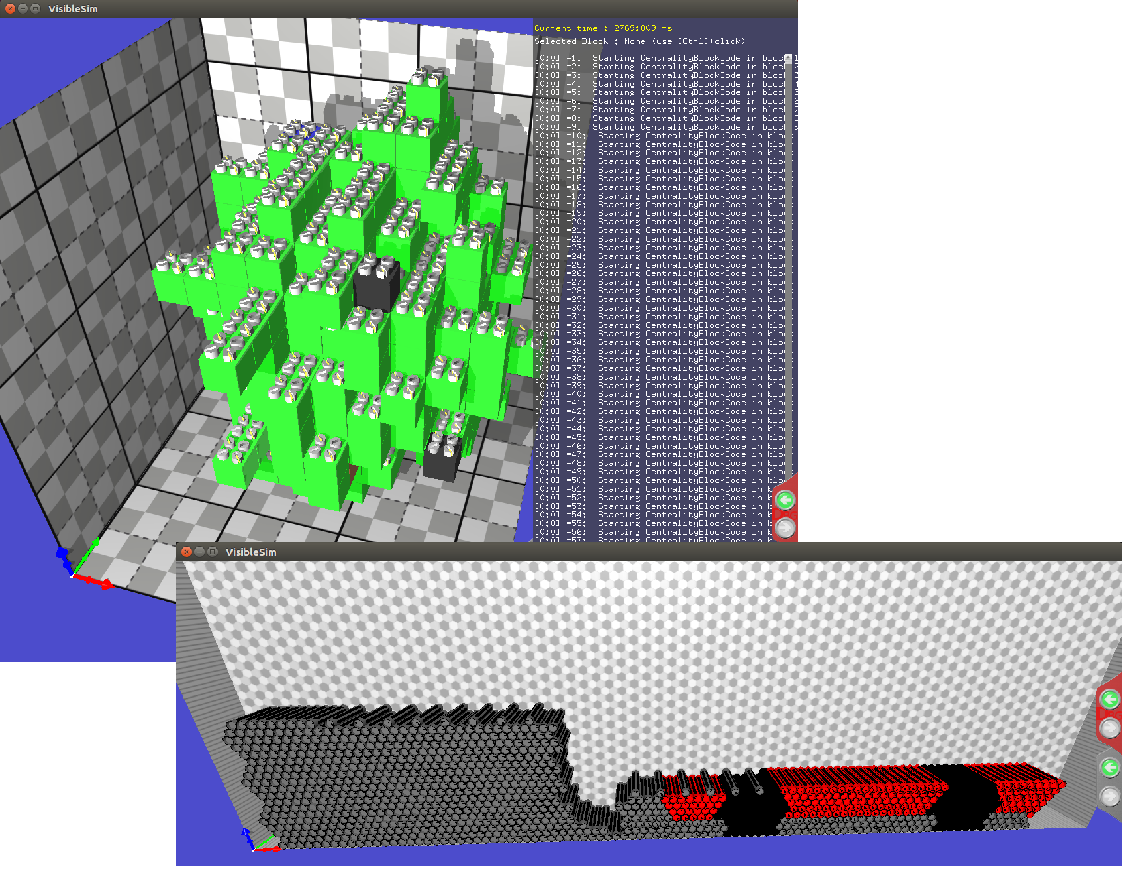
\includegraphics[width=.8\linewidth]{fig/environment/vs}
	\end{center}

\end{frame}
}